\documentclass[a4paper,12pt]{report}
\usepackage[dvips]{color}
\usepackage{lscape}
\usepackage{color}
\usepackage{url}
\usepackage{rotating}
%\usepackage[Sonny]{fncychap}
%\usepackage[Bjarne]{fncychap}
%\usepackage[Lenny]{fncychap}
%\usepackage[Glenn]{fncychap}
\newcommand{\ug}{$\mu g m^{-3}$}

%%% I tried using \bv to start a small-tex verbatim section and
%%% \ev to end this. However, it seems that \end{verbatim} needs to
%%% to be writtehn explcitly, so I use \ev now to end the small-text.
%%% Place directly after \end{verbatim}.

%% \newcommand{\bv}{\begin{small}\begin{verbatim}}
%% \newcommand{\ev}{\end{small}}

\newcommand{\Par}{{\bf Par\_ml}}
\newcommand{\MyOutputs}{{\bf My\_Outputs\_ml}}

\begin{document}
%\begin{landscape}
 
\title{The Unified EMEP Model - User Guide\\
 (draft 1.0)}
\maketitle


\chapter{Welcome to EMEP }

This guide gives a brief documentation of the EMEP/MSC-W model
version rv4.8. 
It is intended primarily as a guide on how to run the model, and
to help users wishing to understand or change 
the model in terms of domains, outputs, chemistry, etc.


The main documentation for the EMEP/MSC-W model is an article pulished 
in Atmospheric Chemistry and Physics in 2012. 
This article will be referred to as Simpson et al. (2012) in
this manual. 


\begin{itemize}
\item
Simpson, D., Benedictow, A., Berge, H., Bergstr\"om, R., Emberson, L.D., Fagerli, H., Flechard, C.R., Hayman, G.D., Gauss, M., Jonson, J.E., Jenkin, M.W., Ny\'iri, \'A, Richter, C., Semeena, V.S, Tsyro, S., Tuovinen, J.-P., Valdebenito, \'A., and Wind, P.:
The EMEP MSC-W chemical transport model – technical description.  
Atmospheric Chemistry and Physics, 12, 7825-7865, 2012.\\
\url{http://www.atmos-chem-phys.net/12/7825/2012/acp-12-7825-2012.html}
\end{itemize}


The model source code is available from the EMEP/MSC-W Open Source website:\\ 
\url{https://wiki.met.no/emep/page1/emepmscw_opensource}

\newpage

\section{Licenses and Caveats}

The EMEP code is provided under the GNU General Public License version 3
(\url{http://fsf.org} and/or
\url{http://www.gnu.org/copyleft/gpl.html}).

Each code module is prefaced with something like:
\begin{quote}
\begin{small}
\begin{verbatim}
! <EXAMPLE_CODE.f90 - A component of the EMEP MSC-W  Eulerian
!          Chemical transport Model>
!*****************************************************************************!
!*
!*  Copyright (C) 2007-2012 met.no
!*
!*  Contact information:
!*  Norwegian Meteorological Institute
!*  Box 43 Blindern
!*  0313 OSLO
!*  NORWAY
!*  email: emep.mscw@met.no
!*
!*    This program is free software: you can redistribute it and/or modify
!*    it under the terms of the GNU General Public License as published by
!*    the Free Software Foundation, either version 3 of the License, or
!*    (at your option) any later version.
!*
!*    This program is distributed in the hope that it will be useful,
!*    but WITHOUT ANY WARRANTY; without even the implied warranty of
!*    MERCHANTABILITY or FITNESS FOR A PARTICULAR PURPOSE.  See the
!*    GNU General Public License for more details.
!*
!*    You should have received a copy of the GNU General Public License
!*    along with this program.  If not, see <http://www.gnu.org/licenses/>.
!*****************************************************************************!
\end{verbatim}
\end{small}
\end{quote}
And a copy of the license file, {\bf gpl.txt}, is provided with the
model code source files.

\noindent It is important to note that the code is provided ``as it is'', 
and EMEP/MSC-W has very limited resources with which to support
code-usage. 

%% To help users an {\bf EMEP Forum} is available from the
%% EMEP/MSC-W Open Source website in section ``Users'': ``EMEP Forum''. 
%% Support to the user community will develop here with your contribution. 
%% Please let us know what your needs for information are 
%% (e-mail: emep.mscw@met.no).

\newpage

\section{Computer Information}
\label{sec:compinf}

To compile the EMEP/MSC-W model you need:\\

\textbf{Fortran 95 compiler}

\textbf{NetCDF Library ($>$4.1.3)}

\textbf{MPI Library ($>$1.0)}\\

It is necessary to compile with double precision reals (8 bytes
reals). The program has been used on computers ranging from a Linux laptop to supercomputers 
(Itanium2 cluster, Intel Xeon cluster, Cray XT4, IBM power5+). It is compatible with all 
compilers tested so far:  Intel, PGI, gfortran, XL fortran. A Makefile is included,  
the path to netcdf (INCL and LLIB) have to be adapted to your machine, and the fortran 
compiler (F90) and flags (F90FLAGS) to the compiler you are using.



The code has been tested with 1 to 1024 CPUs, and scales well (for large grids).  If only one 
CPU is used 1-2 GB memory is required. If more than one,
for example 64 CPUs are used, 200 MB of memory per CPU is enough (in
the case of a 132 X 159 grid size). For runs on more than 32 CPUs, a fast interconnect is 
recommended (infiniband for example), for smaller runs, gigabit ethernet is sufficient. 
It takes $\sim$ 5 hrs on 64*Xeon X5355 (2.66GHz) for 1 year simulation.

When downloading input data in order to do a ``base run'' please make
sure that there are 35 Gb disc space available, especially due to
large meteorology input files. The model can be run for shorter periods, users 
can download meteorology for only the period they are interested in, pluss one day. 
 

\section{Getting Started}


It is recommended to read all the chapters of this EMEP/MSC-W model
User Guide before you start downloading anything from the EMEP/MSC-W Open
Source website.

%% Please register as an EMEP User on the {\bf EMEP Forum}
%% (EMEP/MSC-W Open Source website under ``Users'' section: ``EMEP Forum'')
%% before you start downloading the EMEP/MSC-W model code and/or input
%% data. This will give you access to further communication with the
%% developing team and to the section on ``Questions and Answers''. 


This is what you need to do before you can do a ``base run'' with the 
EMEP/MSC-W model:

\begin{itemize}
%\item Register as an EMEP User
\item Read the EMEP/MSC-W model User Guide
\item
Download input data (description in Chapter~\ref{ch:InputFiles} and
data available from the EMEP/MSC-W Open Source website under ``Download''
section: ``Input Data'')
\item
Download the EMEP/MSC-W model source code (description in 
section~\ref{sec:ModelCode} and the files are available from the EMEP/MSC-W 
Open Source website under ``Download'' section: ``Model Code'')
\item
Follow the instructions for 'Submitting a Run' description in
Chapter~\ref{ch:SubmitARun}.
\item
Download some model results for comparison, description in
Chapter~\ref{ch:output} and the files are available from the EMEP/MSC-W 
Open Source website under ``Download'' section: ``Model Results''. 
%NEWTOOLS:
% \item
% If wanted, download some helper programmes to read site and sonde outputs, 
% see sections~\ref{sec:tools},\ref{sec:sitesonde}.
% The files are available from the EMEP
% Open Source website under ``Download'' section: ``Tools''.


\end{itemize}

\section{Model code}
\label{sec:ModelCode}

The EMEP/MSC-W model code version rv.4.8 are archived as a tar file. 
The tar file is called ``EMEP\_MSC-W\_model.rv4.8.OpenSource.tar.gz'' and 
is downloadable from the EMEP/MSC-W Open Source website.

Once this file is untarred all model files needed for a model run will be 
found under the directory \\ {\bf EMEP\_MSC-W\_model.rv4.8.OpenSource/code/} 
where the model source code, makefiles, and a copy of the license file are 
stored. An overview is given in Table~\ref{Tab:modelfiles}

\begin{table}[h]
\begin{center}
\caption{Contents of ``EMEP\_MSC-W\_model.rv4.8.OpenSource.tar'' file
   \label{Tab:modelfiles}}
\begin{tabular}{ll}
& \\
\hline
Type      & Filename          \\
\hline
& \\
{\bf Model code directory} & EMEP\_MSC-W\_model.rv4.8.OpenSource/code \\ 
\hline
modules files & *.f90 \\
include files & *.inc \\
namelist & config\_emep.nml \\
makefiles & Makefile and Makefile.SRCS \\
dependency file &  dependencies\\
a copy of the license & gpl.txt \\
\hline
\end{tabular}
\end{center}
\end{table}

In addition there is a run script called ``modrun.sh'', which will be placed 
in the \\{\bf EMEP\_MSC-W\_model.rv4.8.OpenSource/}  directory. The run 
script, ``modrun.sh'', can easily be modified to work on your computer system. 
This script is described in detail in Chapter \ref{ch:SubmitARun}. 
 
%NEWTOOLS
% \section{Helper tools}
% \label{sec:tools}
% ????
% For users interested in reading the ascii site and sonde specific outputs,
% two help programmes (Rd\_sites.f90, Rd\_sondes.f90) are provided, 
% in the \\{\bf EMEP\_Unified\_model.OpenSource2012/tools}  directory. These
% programmes are readily compiled with e.g. gfortran, and can be run without
% arguments to obtain usage instructions. See section~\ref{sec:sitesonde}
% for more details.


\section{Model grid}
\label{sec:ModelGrid}

The current EMEP model version, and the provided gridded input data,
have a horizontal resolution of 50$\times$50 km$^2$ (at 60$^\circ$N)
and are defined on a
polar stereographic projection with 20 sigma levels vertically. 
The model is very flexible with regard to the horizontal
resolution, in that it readily makes use of 
meteorological data provided with the model. The vertical
resolution is currently still restricted to the fixed 20 layer
system. The physical
description is given in detail in Chapter 2 of the EMEP Status Report
1/2003 Part I (Simpson {\sl et al.}, 2003).

In 2008 the official EMEP domain was extended eastwards in order to include the 
EECCA countries in the EMEP model grid, see Figure \ref{fig:EECCA}. To distinguish the new grid from the old EMEP 
grid, the new grid is called EECCA in this text and in the config\_emep.nml.

\begin{figure}[ht]
 \centering
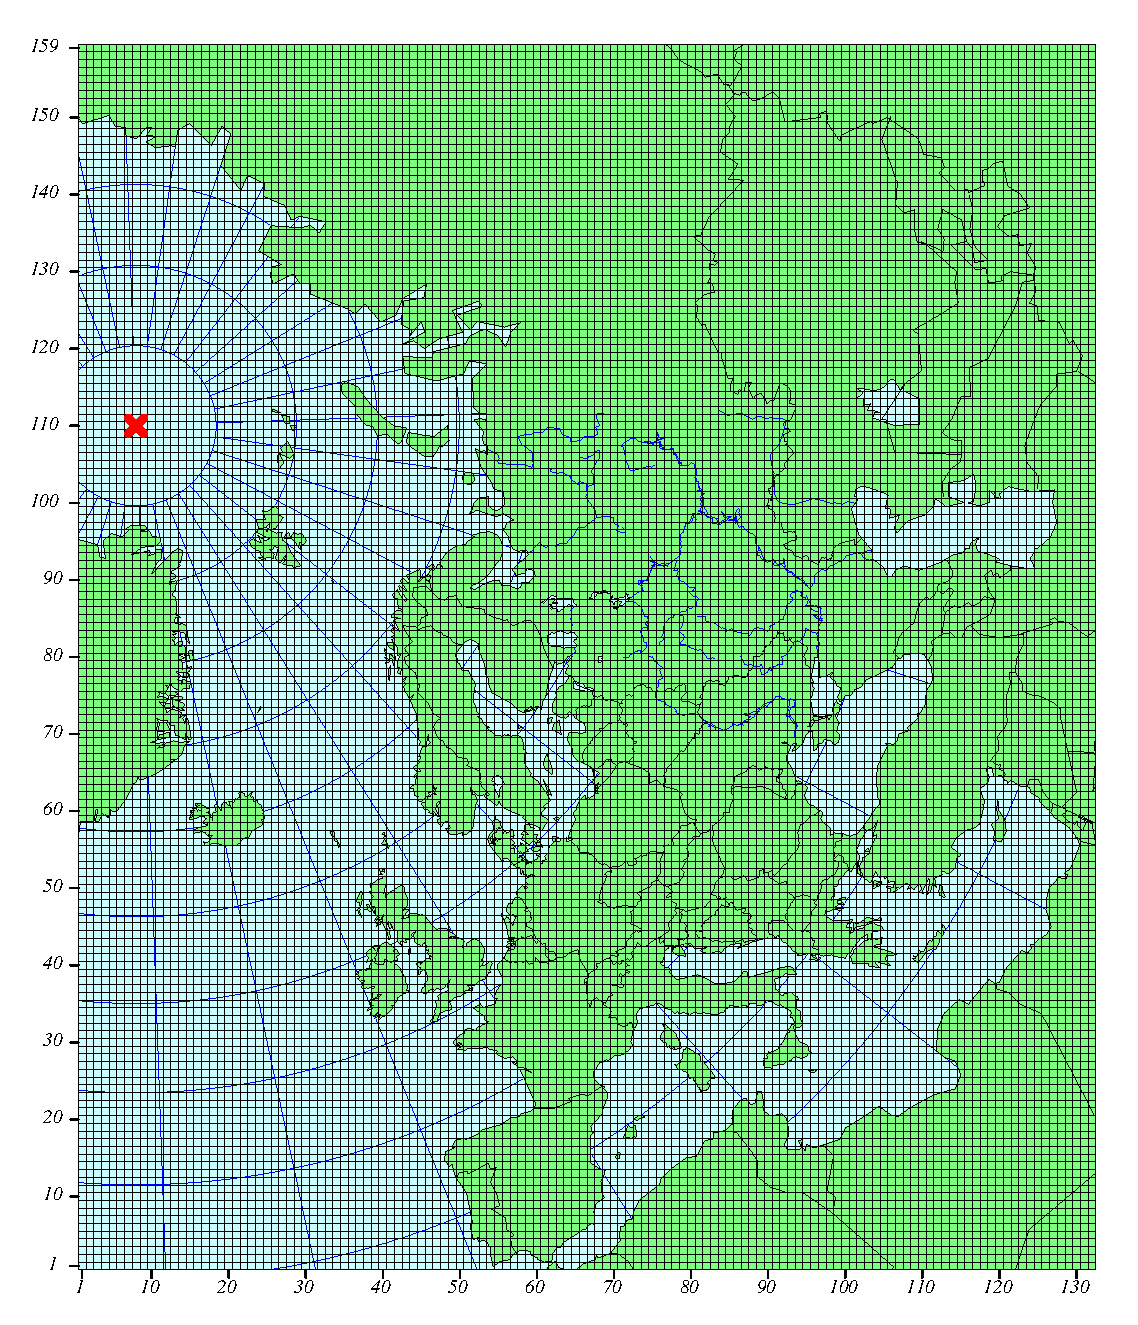
\includegraphics[scale=0.7]{EECCA.eps}
\caption{The extended EMEP grid covering EECCA area with
132$\times$159 gridpoints on 50$\times$50 km$^2$ resolution defined on a polarstereographic
projection.}\label{fig:EECCA}
\end{figure}



%\newpage
\chapter{Domains and Coordinates}

\section{Domains}

Domains - a confusing word. In normal modelling terminology domains
refer to the total area covered by the model simulation, and possibly
to some output areas. In the unified model, and parallel-coding terminology,
domains refer also to the area covered by each processor. To try to distinguish
between these, we generally refer to the former type as `full' domains, 
and the latter as local domains.  At present the `full' domain in the
EMEP model is defined by the meteorology. Thus, for the traditional EMEP
grid this full domain extends 170 grid squares in the x-direction, and
133 grid squares in the y-direction.

The model has a number of domains, illustrated in Fig.\ref{fig:Domains}

\begin{figure}
\begin{picture}(400,300)
\put(2,2){\framebox(340,266)[br]{Meteorology}}
\put(72,20){\framebox(260,240)[br]{EMEP area}}
\put(92,40){\framebox(200,160)[br]{Run area}}
\put(130,60){\dashbox{0.9}(180,180)[br]{Hourly output}}
\put(200,90){\dashbox{0.6}(30,30)[br]{Restri output}}
\end{picture}
\caption{Illustrations of different domains in the EMEP
model.}
\label{fig:Domains}
\end{figure}



\subsection{Full (Meteorology) area} 

Specifies the master coordinates to be used in the model. 
(As noted above, at present the `full' domain and
 meteorology domain are identical).


\noindent
Set in {\bf run.pl} : @largedomain = ( 1 , 171, 1 , 133 );\\
\vspace{3mm}

Translated into \Par\ as:\\
\begin{small}\begin{verbatim}
  integer, public, parameter ::  &
    IILARDOM    =    170         &
  , JJLARDOM    =    133         &
\end{verbatim}
\end{small}



Translated as for Run area (below)

\section{ Run area  (and its shadow!) } 

\noindent
Set in {\bf run.pl} : @smalldomain = ( user-specified  );  \\
\vspace{3mm}
\\
For example, @smalldomain = ( 101, 140, 51, 90 ) 
translates to the following in \Par:\\
\begin{small}\begin{verbatim}
  integer, public, parameter ::  &
  , ISMBEG      =   101    & ! Starting x-coodinate
  , JSMBEG      =   51     & ! Starting y-coodinate
  , GIMAX       =   40     & ! Number of global points in longitude
  , GJMAX       =   40     & ! Number of global points in latitude
\end{verbatim}
\end{small}

The traditional EMEP run area corresponds to  @rundomain = ( 36, 160, 11, 123 ).


The area run by the model does not need to be the EMEP area, just
any sub-domain of the meteorology domain. For testing we could choose just to
have a tiny run-domain. For testing with 4 or 8 processors then
\@smalldomain = ( 51, 160, 31, 120 ) works quite well.



\subsection*{Shadow area}

COULD MOVE THE FOLLOWING TO A PART B, FOR CODING. ONLY REALLY RELEVENT
FOR USERS WHO WANT TO DIG  INTO THE CODE - EXCEPT TO NOTE THAT THERE
IS AN `EDGE' FOR WHICH CALULATIONS AREN'T DONE.

IMPORTANT when coding - the grid cells on the boundaries of the run-area are
excluded from the chemical calculations, since the advection routines
require one cell more than the chemistry. Thus, in \Par\ you will find:

\begin{small}\begin{verbatim}
From par_ml.f90
     limax       & ! Actual number of local points in longitude
   , ljmax         ! Actual number of local points in latitude

     li0  & ! First local index in longitude when outer boundary is excluded
   , li1  & ! Last local index in longitude when outer boundary is excluded
   , lj0  & ! First local index in latitude when outer boundary is excluded
   , lj1    ! Last local index in latitude when outer boundary is excluded
\end{verbatim}
\end{small}


So, if you loop over something that does not need
info from neighboring boxes then it is ok to use li0:li1, lj0:lj1,
but if you need info from the "shadow area" (ie advection)  you must use
1:limax,1:ljmax.
\bigskip
\bigskip


The domains used for the outputs are discussed more in section~\ref{OUTPUTS}.



\subsection{Summary of coordinates}


Table~\ref{Tab:COORDS}
gives an example of the various coordinates and limits for the case of
4 processors (me=0,1,2,3), and a run domain set with:

\begin{verbatim}
@rundomain = (  76, 117,  40, 102 ) ; 
\end{verbatim}

NEED TO EXPLAIN i\_glob, j\_glob, WHY MAXLIMAX+1.

\begin{table}
\caption{Example of coordinates derived for each processor with
the case of 4 processors (me=0,1,2,3) and smalldomain:  76, 117,  40, 102}
For example, processor me=0 covers ..... continue


\label{Tab:COORDS}
\begin{tabular}{lcccc}\\
me& 0& 1& 2& 4\\
ISMBEG& 76& 76& 76& 76\\
JSMBEG& 40& 40& 40& 40\\
gi0& 1& 22& 1& 22\\
gj0& 1& 1& 32& 32\\
li0& 2& 1& 2& 1\\
li1& 21& 20& 21& 20\\
limax& 21& 21& 21& 21\\
MAXLIMAX& 21& 21& 21& 21\\
lj0& 2& 2& 1& 1\\
lj1& 31& 31& 31& 31\\
MAXLJMAX& 32& 32& 32& 32\\
i\_glob(1)& 76& 97& 76& 97\\
i\_glob(MAXLIMAX+1)& 97& 118& 97& 118\\
j\_glob(1)& 40& 40& 71& 71\\
j\_glob(MAXLJMAX+1)& 72& 72& 103& 103\\
\end{tabular}
\end{table}

\chapter{Input files}

This section describes some standard input files for the
EMEP model. In general, the larger input files
are in netCDF format, and the smaller ones in ASCII.
Table~\ref{Tab:Inputs} lists the files used.

\section{NetCDF files}

The Meteorology and Boundary and Initial conditions files are provided
in NetCDF format.  3 hourly meteorological outputs of PARLAM-PS, the
specially dedicated version of the 
operational model HIRLAM is used as the input
meteorology for EMEP.  These are available as daily files. \\

The boundary and Initial conditions file contain the boundary
conditions for the chemical species.  This monthly file contains the
3-D concentration and background concentrations  of the advected
species.  See 'BoundaryConditions\_ml.f90' routine of the model source
code for more details about this data set.  

\section{ASCII files}

All other files including the emissions, landuse, snowcover etc., are
in ascii format.  
We have started recoding the model  and inputs
to allow more header information in Ascii files (section~\ref{sec:NewInputs}), 
but so far only 6 files have
this new-style. For other files it may be necessary to read the
appropriate Fortran module in order to understand the formats and usage.

\subsection{`Standard-style' inputs}

Gridded emission files contain 16 columns where the first column
represents the country code, the second and third are the 'i' and 'j'coordinates of the model grid, the fourth and fifth are the total emissions from
low (below 100 m of the model level, mainly from traffic,
agricultural emissions etc.,) and high sources (above 100 m of the
model level, which are from industry, power plants etc.),
and the rest 11 columns contain anthropogenic emissions from 10 SNAP1
emission sectors (Source-Nomenclature for Air Pollution) and natural emissions. 
(Note that natural emissions for BVOC should \emph{not} be included
in these files, but are calculated from the Inputs.BVOC information).
Sector means
the source type of emissions from each country and there are 11
sectors defined in EMEP.  A listing of all type
of sectors are given in 'EmisDef\_ml.f90' of the model source code.   An arbitrary
example file would look like  \\

\textbf{An example emission file:}
\begin{verbatim}

#countrycode i j low high sectors1 2 3 4 5 6 7 8 9 10 11 
1 1 4 20.8 1.0 0.0 7.9 0.6 0.0 0.0 0.0 6.4 4.1 0.8 0.0 0.0
1 1 5 24.0 0.0 2.5 5.7 0.8 0.0 3.0 5.0 4.4 2.1 0.5 0.0 0.0
1 1 7 29.7 0.0 5.5 8.9 0.6 0.0 0.0 0.0 8.4 5.1 1.2 0.0 0.0
...................
etc..........

\end{verbatim}
Climatalogical snowcover (simply zero for absent  or 1 for present) 
 and Natural SO2 emissions are provided as monthly gridded
files and they are stored in columns of 'i', 'j', and the 12 monthly
'values'. 

The file rough.170 contains some roughness lengths from the NWP model
supplying meteorolgoical data to EMEP. We use this to assign a land/sea
mask within the EMEP model, since we modify stability information
for coastal grid cells (which contain land, but where this isn't
resolved by the NWP model).
 

To consider the volcanic emissions, we need to feed the location and
height of volcanoes into the model.  This is provided with the
'Volcanoes.dat' file and the columns in this file represent the 'i'
and j' indexes of the model grid and the third column represent the
model level where the mouth of the volcanoe stands, based on their
height.  The input file contains only two volcanoes which are the only
active volcanoes in Europe.  You might notice that 'Etna, Italy'
appears twice in the input file, which is due to its large base area
it shares two grids in the model.  \\
     


NO$_{x}$ emissions from Aircraft and lightning are also included in the
model. Seasonal commercial aircraft emissions and annual military
aircraft emissions are read in as gridded data from the same file.  Aircraft emissions are tabulated on a 128x64 longitude latitude grid with 16 vertical levels. The grid has global coverage and the values are interpolated to the actual grid.
 The lightning emission are defined on a 64x32 grid with 17 vertical
 levels, with global coverage and are provided as monthly files for the whole
year.      \\

Time factors for emissions depending on the chemical compound, sector,
and country for day of the week and month of the year are provided with
the 'DailyFac.pollutnat' and 'MonthlyFac.pollutant' files.  Data are
stored in columns of 'i','j', factors corresponding to each day of the
week in 7 consecutive columns in case of DailyFac file and factors
corresponding to each month of the year in 12 consecutive columns in
case of MonthlyFac file.\\  

The model also need a split file for some of the emission files.  For
example, only one emission file is provided for NO$_{x}$.  The amount of
NO$_{2}$ compared to other NO is determined by the split file.  It is
land and sector dependent.  The same is true for VOC, but
there are more VOC types present. \\ 

Finally the 'femis.dat' file is provided for setting up a 'scenario run'.  See
chapter 4, 'Submitting a run' for the details about this file.  

 
\bigskip
\subsubsection{New-style  Ascii inputs}
\label{sec:NewInputs}

 The new-style of  input files (which we started to introduce during summer-autumn 2007)
are designed to read nicely in gnumeric and other spread-
sheets (excel, oocalc), and can be either space or comma separated.
Fortran is quite flexible in its reading of separated data, and
would not distinguish between any of:
\begin{verbatim}
2001  7 23  1.2   2.3
2001,7,23,1.2,2.3
2001, 7, 23,   1.2,2.3
2001, 7, 23,   1.2, 2.3
\end{verbatim}

Whereas some spreadsheets get confused if both spaces and commas
are used. It is suggested that files are kept as 
pure comma-separated,
pure space-separated,
or with separation with both comma and space (as in line 4 above).
\bigskip

Lines starting with `:' are for key-value pairs, e.g. : year 2002
The line ending in `\#HEADERS' should contain the headings of each column.
\bigskip

{\bf IMPORTANT:} One line of column headers *must* be provided with this
new-style inputs, and the
 number of headers (excluding commented out ones)  must match the number of data items.
(Any further header lines, e.g. for units, must be commented out, either with
a starting \# or ending \#SKIP).
 All lines starting `\# ' are ignored. The text will show up nicest in
 spread sheets if enclosed in quotation marks, as in line 1 of the example.

\begin{table}[h]
\caption{Input Files}
\label{Tab:Inputs}
\begin{tabular}{p{6cm}ccc}\hline
Data & name (in F90 code) & format\\ \hline
   & & \\
\multicolumn{3}{l}{\bf Netcdf} \\
Meteorology&filNNNN&NetCDF\\
Boundary/Initial Values&Boundary\_and\_Initial\_Conditions.nc&NetCDF\\
   & & \\
\multicolumn{3}{l}{\bf Standard-style Ascii} \\
%LOGAN BC&&&&not used?\\
Snow cover&snowcMM.dat&i j x\\
NWP roughness (for land/sea mask) &  rough.170 & i j x\\
Emissions&gridPOLL&i j x1-x13\\
Natural SO$_{2}$&natso2MM.dat&i j x\\
Volcanoes&Volcanoes.dat&i j k   \\
Time series for emissions&MonthlyFac.POLL&EMEP\\
Time series for emissions&DailyFac.POLL&EMEP\\
Lightning&lt21\_nox.datMM&??& \\
Aircraft&amilt42-nox.dat&??&\\
VOC Splits&vocsplit.defaults&ascii \\
NO$_{x}$ Splits& noxsplit.defaults&ascii\\
femis.dat & femis.dat    & ascii  \\
   & & \\
\multicolumn{3}{l}{\bf New-style Ascii} \\
Land cover(\%) & Inputs.LandData& See headers \\ 
Landcover defs& Inputs.LandDefs& See headers \\ 
Stomatal conductance inputs& Inputs\_DO3SE.csv & See headers \\ 
Biogenic VOC Potentials&Inputs.BVOC& See headers \\
Site locations for ascii output& sites.dat& See headers \\
Sonde locations for ascii output& sondes.dat& See headers \\
\hline
\end{tabular}
Note: Gridded Input Files. NNNN: number, MM: month, POLL: pollutant, AA: text\\
\end{table}


Landuse data are required in the model, primarily for dry
depositon modelling.  EMEP
model can accept landuse data from any dataset covering the whole of
the domain and providing reasonable resolution of vegetation
categories.  Gridded data-sets providing these landuse categories
across the EMEP domain have been created based on the data from the
Stockholm Environment Institute ar York (SEI-Y) and form the
Coordinating Centre for Effects (CCE).These data are contained in the file Inputs.Landuse. The headers of this file contain short abbreviations for the different landcover types, e.g. CF for temperate/boreal coniferous forest.  \\

 16 basic landuse classes have
been identified for the use of deposition module in the model and they
are Temperate/boreal coniferous forests (CF), Temperate/boreal
deciduous forests (DF), Mediterranean needleleaf forests (NF),
Mediterranean broadleaf forests (BF), Temperate Crops (TC),
Mediterranean Crops (MC), Root Crops (RC), Seminatural/Moorland (SNL),
Grassland (GR), Mediterranean Scrub (MS), Wetlands (WE), Tundra (TU),
Desert (DE), Water (W), Ice (I), and Urban (U).  They are listed in
columns following the 'i' and 'j' indexes of the
grids. Three additonal "fake" land-use classes are used for providing results for integrated assessment modelling and effects work . Input file header explains in detail about all the
columns. \\

{\bf IMPORTANT:} The landcover codes found in Inputs.Landuse are taken as 
the definition of landcover. The files Inputs.LandDefs and Inputs\_DO3SE.csv
must have exactly the same codes.\\

For the vegetative landuse categories for which stomatal modelling is
undertaken, the start and end of the growing season (SGS, EGS), as well as
other biomass characteristics, and parameters for the stomatal conductance
model must be specified. This is done in the files Inputs.LandDefs and
Inputs\_DO3SE.csv, and using some functions, e.g. Growing\_season from
LandDefs\_ml.f90.

'Inputs.BVOC' file provide the biogenic VOC emission potentials (i.e.
rates at 30 deg C and full sunlight, see headers for more information).  They
are provided in 4 columns, being the first and second columns as usual
represent the 'i' and 'j' indexes of the model grid and the third and
fourth columns represent the isoprene and terpene emission potentials in unit of
``$ug/m^{2}/h$''.\\


\chapter{Outputs}
\label{OUTPUTS}

%%%%%%%%%%%%%% Sites and Sondes %%%%%%%%%%%%%%%%%%
%%%%%%%%%%%%%%%%%%%%%%%%%%%%%%%%%%%%%%%%%%%%%%%%%%%%%%%%%%%%%%%%%%%%%%%%%%%%%%
\section{sites and sondes}
\label{Output:ascii}

Two main options are available for the output of ascii files for comparison
with measurements or detailed model analysis. These are

\begin{description}
\item[sites]  

      output of surface concentrations for a set of specified
      measurement site locations.
\item[sondes] 

      output of concentrations for the vertical column above
     a set of specified locations.
\end{description}

Both sites and sondes are specified and handled in similar ways, in
the module {\bf Sites\_ml}, so we treat them both together below.

Locations are specified in input files, sites.dat and sondes.dat, whose
directory-locations should be specified in {\bf run.pl}. For example,
a sites.dat file might look like:

\begin{small}\begin{verbatim}
schauinsland    101   51
thessaloniki    132   58
ispra           106   48      Comment: 45.8,8.6333-> 105.864 47.742  (to150old)
testsitemid     120   70      ... just for testing
testsite12      102   88      ... just for testing
border_72_84     72   84      ... just for testing
\end{verbatim}
\end{small}


These file are optional.

The species and meteorological data required are specified in {\bf My\_Outputs}
through the use of arrays. Only a few met fields are defined so far but
more can be added into {\bf Sites\_ml} as required. The outputs consist
of a header giving the number of sites used, species/met data used, and
then actual values specified with a 5es10.3 format. For the sonde data
values are given for all 20 levels, starting with the ground-level values.




%%%%%%%%%%%%%% Hourly %%%%%%%%%%%%%%%%%%%%%%%%%%%%
Output files are written out in NetCDF format.  
Model will write the output files into your working directory (see the
runscript 'run.pl' where you have set the working directory
path. Chapter 4, 'Submitting a Run' explains all the paths).  For a
base run, all the outputs will be stored into a subdirectory called
'Base' under your working directory, and the files will be named
'Base\_day.nc', 'Base\_hour.nc' etc., for a daily output and hourly
output respectively.  You can also provide a better self descriptive
name for the experiments and then the outputs will be written out with
this experiment name as the base name. This is done in the run
script (ref. Chapter 4).  

\section{Hourly out}

\noindent
Optional -  specify in \MyOutputs\, hourly\_out\%ix1, etc.\\
Ascii and netCDF.  Only netCDF outputs will be available in future. 
Put 'Hourly\_ASCII' switch defines whether the output has to be written
into Ascci format or netCDF format.  Ascii may be easy to use, but
produces very large output files.  

\vspace{1cm}

This output is intended to allow hourly (or any resolution) outputs of surface
as well as 3D concentrations in
variable precision for user-defined areas.  

Make sure that the labels 'NHOURLY\_OUT, NLEVELS\_HOURLY, and FREQ\_HOURLY' are updated with the number of
variables, number of levels and frequency of output interval you want
to output into hourly file.  It is explained clearly in the code as
well.  

 
In \MyOutputs\ we have for example:

\begin{small}
\begin{verbatim}
  !**          name type ofmt ispec ix1 ix2  iy1 iy2 nk unit conv max

  hr_out(1) = Hr_output("o3_3m","ADVppbv", 
             "(f8.4)",IXADV_O3, 87, 110, 51, 75,1,"ppbv",PPBINV,600.0)
  hr_out(3) = Hr_output("o3_50m","BCVppbv",
             "(f8.4)",IXADV_O3, 87, 110, 51, 75,20,"ppbv", PPBINV,9000.0)
\end{verbatim}
\end{small}

The above example gives both 3D as well as surface concentration of
Ozone.  Here the type 'ADVppbv' gives surface concentration (note
that nk=1) and 'BCVppbv' gives 3D concentration for all the 20 levels
(nk=20). These are defined in {\bf 'Output\_hourly'}.  The area for which we want to write out the output is
specified with 'ix1','ix2','iy1' and 'iy2'.  Unit is chosen as 'ppbv'
and the conversion factor, 'PPBINV' is coming from
{\bf 'ModelConstants\_ml}'.  


\section{Restricted output}
(TO BE REMOVED! Same functionality available with either use of
sondes files or use of Derived.)

\noindent
Optional -  specify in \MyOutputs\, hourly\_out\%ix1, etc.\\
Binary
\vspace{1cm}

This output is intended to allow 3-hourly (??) outputs of the 3-D concentration
fields for a limited area, for example Milan. Can thus provide boundary-values
for input to other models. (These could also be provided by specifying the
coordinates of the required boundary in the sites.dat file)

In \MyOutputs\ we have for example:

\begin{small}
\begin{verbatim}
  integer, public, parameter ::  &
	 ISPEC_OUTBEG  = 121  &
	,JSPEC_OUTBEG  =  61  &
	,ISPEC_OUTEND  = -130 &     ! Set negative here to exclude
	,JSPEC_OUTEND  = -80        ! Set negative here to exclude
\end{verbatim}
\end{small}


\section{Derived fields and binary outputs}

{\bf modules My\_Derived\_ml, Derived\_ml}\\

My\_Derived\_ml:\\
\begin{itemize}
  \item Constructs arrays wanted\_deriv2d, wanted\_deriv3d, listing
   the outputs which the user wants in netcdf fields.
\end{itemize}

Derived\_ml:\\
\begin{itemize}
  \item Contains definitions of possible output fields
  \item Allocates data arrays d\_2d and d\_3d for those
    fields which were requested in My\_Derived\_ml	
\end{itemize}



\noindent
The fields which are output as netCDF data from model runs consist
of either 2-D or 3-D  arrays, with some identfiers. 
Some data-fields will contain concentration, others depositions, still
others user-defined fields such as column sulphate or AOT40.
Some data will be averaged and printed out daily, other data will
be accumulated to monthly or yearl average totals.
The unified model 
attempts to deal with the various possible data-fields through
a consistent methdology, treating all of the above as simply "derived"
fields.

The basic idea is that  the module Derived\_ml contains an extensive
set of pre-defined outputs. The user chooses which of these
outputs to use by simply defining the arrays wanted\_deriv2d
and wanted\_deriv3d in My\_Derived\_ml.  For example,
we might just have wanted\_derivd2d = (/ "WDEP\_SOX", "D2\_UNAOT40" /)
\footnote{Actually, we usually define wanted\_deriv2d to be
a longer array, and use a string "NOT\_SET\_STRING" to mark
the unwanted elements, thus wanted\_derivd2d = 
(/ "WDEP\_SOX", "D2\_UNAOT40", NOT\_SET\_STRING, NOT\_SET\_STRING, \dots /).
}




A fortran'90 type, Deriv, is defined which contains
a description of the parameters associated with each wanted field.
In this module, derived fields are identified by a "class", such as "ADV" of "VOC".
The user also specifies if averaging is wanted, and sets various
time markers to be true or false. More details are supplied below.

 The Derived\_ml should perform any integrations for these fields.
 Several often-used routines (e.g. for AOTs, acc. sulphate, are defined 
 in the Derived\_ml.f90, and these are only called if the appropriate
 class is found from My\_Derived\_ml. (Users should also be
 able to define their own routines in My\_Derived\_ml, since
 we do not use "use only" in Derived\_ml. However, as far as possible
 we are trying to to keep My\_Derived short and the routines flexible.)

  We define 4 possibilities
  for output time-periods, corresponding to: instantaneous,year,month,day:

  \begin{small}\begin{verbatim}
   integer, public, parameter ::  NIOUTYP = 4
   integer, public, parameter ::  & 
        IOU_INST=1, IOU_YEAR=2, IOU_MON=3, IOU_DAY=4
  \end{verbatim}
  \end{small}


   We also define a new type,`Deriv':

  \begin{small}\begin{verbatim}
    type, public:: Deriv
       character(len=5) :: class ! Class of data, e.g. ADV or VOC
       logical  :: avg      ! True => average data (divide by nav), else accumulate
       integer  :: index    ! index in concentation array, or other
       real     :: scale    ! Scaling factor          ! (was SCALOUT_DERIV_3D)
       logical  :: inst     ! True when instantaneous values needed
       logical  :: year     ! True when yearly averages wanted
       logical  :: month    ! True when monthly averages wanted
       logical  :: day      ! True when daily averages wanted
    end type Deriv
  \end{verbatim}
  \end{small}


  By using this Deriv type, and the subroutine AddDef which sets the elements of the
  Deriv arrays
  def\_2d, def\_3d to be equal to the routines input arguments, we can specify the characteristics of the data
  with just one line of fortran. For example, for the wet deposition of
  sulphur oxides, we use:


  \begin{small}
\begin{verbatim}
    call AddDef("WDEP ", F, -1, 1.0e6, F  ,  T , T ,  T, "WDEP_SOX","mgS/m2")
  \end{verbatim}
  \end{small}

  (Note, F is shorthand for false, T for true.)\\
  \bigskip


 \noindent
  And if WDEP\_SOX is asked for in the My\_Derived list, the Derived\_ml will
  set one of the f\_2d fields to match the above.
  For this example, WDEP\_SOX is the text field we need to identify the
  data, and we set a scaling factor of 1.0e6 for output. The index
  is set to -1 since we do need access to any one index from say 
  the xn\_adv arrays.
   The class
  "WDEP" will tell the rest of the code that this is a wet-deposition field,
   and  calculations will be done accordingly. 

   We have set the avg field to false, as wet-deposition needs to be accumulated,
   not averaged. The time fields show that we want daily, monthly and yearly
   output, but not output of instantaneous fields.

   \begin{table}[h]
   \caption{Summary of parameters, definition and data arrays for derived types}
   \label{TABDRV}
   \begin{tabular}{|lllp{6cm}|}\hline
     No. fields    &  Definition array & Data array  & Comments  \\
                   &               &                 &           \\
     NWDEP         &    f\_wdep    &    wdep   & Wet deposition and accumulated precipitation  \\
     NDDEP         &    d\_wdep    &    ddep   & Dry deposition   \\
     NDERIV\_2D     &    f\_2d      &    d\_2d   & Derived 2-D fields, surface concs., etc.  \\
     NDERIV\_3D     &    f\_3d      &    d\_3d   & Derived 3-D fields  \\ \hline
   \end{tabular}
   \end{table}

%
% More coding comments .....
\chapter{Model structure}

The model is composed of a large number of modules together with a few
standalone subroutines. The intention is that \emph{only}
modules which are prefixed `{\bf My\_}'  should change for different
model versions. Thus, changing from ozone to acidification models
should consist of changing only these modules. It is envisaged that
in future such My\_ files can be collected into separate directories
and loaded into the main model direcory when required.

Files which do not begin with `My\_' should not need to be changed
at all for different model versions. Think very carefully before
making any changes here - there will hopefully be an option to
do what you want  in the My\_ files!! If not, we need to create
such an option, or persuade you to make do with another method ;-)


Currently, two sub-directories, {\bf ZD\_OZONE} and {\bf ZD\_ACID}
are used to store the various `My' files. SImply copy these
into the main directory befor compilation to get the version required.

\begin{small}
\begin{table}
\caption{The Unified model files}
\begin{tabular}{|llll|} \hline
Unimod.f90  &                      &                    &  \\
\hline
BoundaryConditions\_ml.f90 & My\_BoundConditions\_ml.f90 & UiO\_ml.f90  &  \\
\hline
Chem\_ml.f90 &  My\_Chem\_ml& My\_Reactions.in  &  \\
Aqueous\_ml.f90 &  &   &  \\
Ammonium\_ml.f90 &  &   &  \\
DefPhotolysis\_ml.f90 &  &   &  \\
DryDep\_ml.f90     & My\_DryDep\_ml &   &  \\
WetDep\_ml.f90     & My\_WetDep\_ml &   &  \\
OrganicAerosol\_ml.f90 &  &   &  \\
Runchem\_ml.f90 &  &   &  \\
Solver.f90 &  &   &  \\
\hline
EmisGet\_ml.f90 & My\_Emis\_ml.f90 & EmisDef\_ml.f90  &  \\
Emissions\_ml.f90 &  &   &  \\
Biogenics\_ml.f90 &  &   &  \\
AirEmis\_ml.f90 &  &   &  \\
Timefactors\_ml.f90 &  &   &  \\
\hline
ModelConstants\_ml.f90 &  &   &  \\
PhysicalConstants\_ml.f90 &  &   &  \\
\hline
Io\_ml.f90 &  &   &  \\
NetCDF\_ml.f &  Derived\_ml.f90 & My\_Derived\_ml.f90  &   \\
Output\_hourly.f &  My\_Outputs\_ml.f90 &   &  \\
Out\_restri\_ml.f90 &  &   &  \\
outchem\_restri.f &  &   &  \\
Sites\_ml.f90 &  &   &  \\
\hline
%gc\_com.F &  & Par\_ml   &  \\
%getflti2.F &  &   &  \\
%parinit.f &  &   &  \\
%putflti2.F &  &   &  \\
%put\_restri\_i2.F &  &   &  \\
%\hline
Advection\_ml.f90 &  &   &  \\
Bud\_ml.f90 &  &   &  \\
Country\_ml.f90 &  &   &  \\
Dates\_ml.f90 &  &   &  \\
Functions\_ml.f90 &  &   &  \\
GridValues\_ml.f90 &  &   &  \\
Met\_ml.f90 &  &   &  \\
Polinat\_ml.f90 &  &   &  \\
Setup\_1d\_ml.f90 &  &   &  \\
Setup\_1dfields\_ml.f90 &  &   &  \\
Tabulations\_ml.f90 &  &   &  \\
\hline
gc\_com.F &  & Par\_ml   &  \\
getflti2.F &  &   &  \\
parinit.f &  &   &  \\
putflti2.F &  &   &  \\
put\_restri\_i2.F &  &   &  \\
\hline
global2local.f &  &   &  \\
local2global.f &  &   &  \\
phyche.f &  &   &  \\
zenit\_angle.f &  &   &  \\
\hline
\end{tabular}
\end{table}
\end{small}



\chapter{The Code}



\begin{itemize}
\item
95\% Fortran 90/95

\item
Preferably in F
   \begin{itemize}
      \item
        A sub-set of F95
   \end{itemize}

\item
   Heavy use of 'modern' fortran and modules
   \begin{itemize}
      \item
        e.g. No common blocks
      \item
        intent attributes  in subroutine arguments
   \end{itemize}
\end{itemize}

\section*{A simple module}

\begin{verbatim}
      module PhysicalConstants_ml
!----------------------------------------------------------------------------
!  Defines Physical constants
!----------------------------------------------------------------------------
implicit none
private

  real , public, parameter ::         &
    AVOG   = 6.023e23                 & ! Avogadros number
  , ATWAIR = 28.964                   & ! mol wt of air, g/mol
  , RGAS_ATML = 0.08205               & ! Molar Gas constant (atm M-1 K-1)
  , RGAS_KG   = 287.0                 & ! Molar Gas constant (J K-1 kg-1)
  , RGAS_J    = 8.314                   ! Molar Gas constant (J mol-1 K-1)

  real, public, parameter  ::    &
       GRAV    = 9.807           &   ! Gravity, m s-2
  ....
    ,  FREEPATH  = 6.5e-8        &   ! Mean Free Path of air [m]
  ....

\end{verbatim}



%\newpage
To use, e.g.  AVOG from another module, one usually uses:

\begin{verbatim}

module Demo1
  use PhysicalConstants_ml, only : AVOG
 ...
end module Demo1

\end{verbatim}

More complex modules mix subroutines and data.


A typical EMEP code module looks like
\begin{verbatim}

module Demo2
  use PhysicalConstants_ml, only : AVOG
  use Rsurface_ml,  only : Rsurface, Gsto, Rb
 ...

  !/ Subroutines:

  public :: demo_sub
  private :: Initialise
  private :: Tabulate


  logical, save, private :: my_first_call = .true.

 contains
   subroutine demo_sub(a,b,c)
     real, intent(in) :: a, b
     real, intent(out) :: c

     if ( my_first_call ) then
           call Initialise
           call Tabulate
           my_first_call = .false.
     end if

     call Rsurface(....)

   end subroutine demo_sun

   subroutine Initialise
      bla bla 
   end subroutine Initialise

   subroutine Tabulate
      bla bla 
   end subroutine Tabulate

end module Demo1

\end{verbatim}

%\newpage
\chapter{Model architecture and variable names}

The picture below ilustrates the vertical structure of the model. The model 
is using sigma coordinates. There are 20 vertical layers from 100 hPa to 
the surface in the model. z\_bnd denotes the devision between the layers 
(z\_bnd(1) is the height of the top of the model and z\_bnd(21) the surface.
z\_mid(1) is the height of the midpoint of the top layer and z\_mid(20) the 
height of the mid point of the lowest model layer.

\begin{picture}(400,300)
\linethickness{0.5mm}\scriptsize
\multiput(0,25)(0,50){6}{\line(1,0){250}}
\linethickness{0.25mm}\scriptsize
\multiput(0,50)(0,50){5}{\line(1,0){100}}
\put(140,10){\makebox(0,0){\large Surface}}
\put(320,20){\makebox(0,0)[b]{{\large z\_bnd(KMAX\_BND) }}}
\put(330,70){\makebox(0,0)[b]{{\large z\_bnd(KMAX\_BND - 1) }}}
\put(330,120){\makebox(0,0)[b]{{\large z\_bnd(KMAX\_BND - 2) }}}
\put(330,170){\makebox(0,0)[b]{{\large z\_bnd(KMAX\_BND - 3) }}}

\put(190,195){\makebox(0,0)[b]{{\large z\_mid(KMAX\_MID-3) }}}
\put(190,145){\makebox(0,0)[b]{{\large z\_mid(KMAX\_MID-2) }}}
\put(190,95){\makebox(0,0)[b]{{\large z\_mid(KMAX\_MID-1) }}}
\put(180,45){\makebox(0,0)[b]{{\large z\_mid(KMAX\_MID) }}}
\end{picture}
\vskip 5 mm

In the horizontal the model use a 50x50 km polar stereographic mapping, 
true at 60$^{\circ}$N. 
The horizontal topography is ilustrated in the picture below by the 
south-west corner of the 
model domain. The horizontal vinds (u and v) are given on a staggered grid 
(this is also the case with the vertical vind component sdot). All other 
variables (represented as q in the picture) are given in the centre of the 
grid.

\begin{picture}(400,250)
\linethickness{0.5mm}\scriptsize
%draw the lines
\multiput(30,30)(0,75){3}{\line(1,0){300}}
\multiput(30,30)(75,0){5}{\line(0,1){150}}
%make the dots
\put(67,67){\circle*{2}}
\put(142,67){\circle*{2}}
\put(217,67){\circle*{2}}
\put(292,67){\circle*{2}}

\put(67,142){\circle*{2}}
\put(142,142){\circle*{2}}
\put(217,142){\circle*{2}}
\put(292,142){\circle*{2}}
%write u,v - old version incorrect!!
%\put(30,10){\makebox(0,0)[b]{{\large u,v$_{(0,0)}$ }}}
%\put(105,10){\makebox(0,0)[b]{{\large u,v$_{(1,0)}$ }}}
%\put(180,10){\makebox(0,0)[b]{{\large u,v$_{(2,0)}$ }}}
%\put(255,10){\makebox(0,0)[b]{{\large u,v$_{(3,0)}$ }}}
%
%\put(0,105){\makebox(0,0)[b]{{\large u,v$_{(0,1)}$ }}}
%\put(0,180){\makebox(0,0)[b]{{\large u,v$_{(0,2)}$ }}}

%New, following Peter's sketch:
\put(10,60){\makebox(0,0)[b]{{\large u$_{(0,1)}$ }}}
\put(10,135){\makebox(0,0)[b]{{\large u$_{(0,2)}$ }}}
\put(72,10){\makebox(0,0)[b]{{\large v$_{(1,0)}$ }}}
\put(147,10){\makebox(0,0)[b]{{\large v$_{(2,0)}$ }}}
\put(222,10){\makebox(0,0)[b]{{\large v$_{(3,0)}$ }}}
\put(297,10){\makebox(0,0)[b]{{\large v$_{(4,0)}$ }}}


\put(67,50){\makebox(0,0)[b]{{\large q$_{(1,1)}$ }}}
\put(142,50){\makebox(0,0)[b]{{\large q$_{(2,1)}$ }}}
\put(217,50){\makebox(0,0)[b]{{\large q$_{(3,1)}$ }}}
\put(292,50){\makebox(0,0)[b]{{\large q$_{(4,1)}$ }}}

\put(67,125){\makebox(0,0)[b]{{\large q$_{(1,2)}$ }}}
\put(142,125){\makebox(0,0)[b]{{\large q$_{(2,2)}$ }}}
\put(217,125){\makebox(0,0)[b]{{\large q$_{(3,2)}$ }}}
\put(292,125){\makebox(0,0)[b]{{\large q$_{(4,2)}$ }}}

\end{picture}


In the tables below the most important variable names used in the Unified 
model will be listed. For some parameters a reference will be given to other 
sections of the documentation in the ``ref.'' column in the tables.


\begin{table} [h]
\begin{center}
\caption{Meteorological input data. The data are in general intentaneous 
values unless listed as 3 h avg. in the dimension column in wich case the 
variable is givea as a 3 hour average.}
\label {table:variable_inmet}
\begin{tabular} {l|l|l|l|l}
Variable name & description             &dimension& unit       & ref.   \\
\hline
u             & vind in x - dirrection  & 3 d   & m s$^{-1}$   &        \\
v             & vind in y - dirrection  & 3 d   & m s$^{-1}$   &        \\
sdot          & vertical vind component & 3 d   & Pa s$^{-1}$  &        \\
th            & potential temperature   & 3 d   & Deg. K       &        \\
q             & specific humidity       &3 d    & mass ratio &        \\
cw            & cloud water            & 3 d, 3 h avg.& kg$_w$/kg$_{air}$  & \\
cc3d          & cloud cover 3 h average & 3 d, 3 h avg.& percent   &        \\
pr            & 3 h precip. summed from abv.& 3 d, 3 h avg. & kg m$^{-2}$ &  \\
ps            & surface pressure        & 2 d   & Pa           &        \\
th2m          & teperature at 2 m       & 2 d   & Deg. K       &        \\
fh            & surface flux sens. heat & 2 d   & W m$^2$      &        \\
fm            & surface stress          & 2 d   & N m$^2$      &        \\ 

\end {tabular}
\end {center}
\end {table}


\begin{table} [h]
\begin{center}
\caption{Derived meteorological data.The data are in general intentaneous 
values unless listed as 3 h avg. in the dimension column in wich case the 
variable is givea as a 3 hour average.}
\label {table:variable_derivmet}
\begin{tabular} {l|l|l|l|l}
Variable name & description             &dimension& unit       & ref.   \\
\hline
roa           & density                 & 3 d     & kg m$^{-3}$&        \\
cc3dmax       & max. cloud cover above  & 3 d, 3 h avg. & percent  &      \\
p1            & pressure at sigma\_bnd   & 3 d     & Pa         &        \\
z\_bnd         & height at sigma\_bnd     & 3 d     & m          &        \\
z\_mid         & height at sigma\_mid     & 3 d     & m          &        \\
skh           & exhange coefficient     & 3 d     & ??         &        \\
\end {tabular}
\end {center}
\end {table}


%\newpage
\chapter{Programming rules and tips}


The mixed FORTRAN'77 - FORTRAN'90 code of the earlier models
has been extensively replaced by pure FORTRAN'90. The biggest change
is in the use of modules instead of include-files and common blocks
to share data and subroutines between different parts of the model.
One advantage of mouldes is that it allows the explicit statement
of thre variables which are being used. Thus, 

\begin{verbatim}
use PhysicalConstants_ml, only : KARMAN
\end{verbatim}

\noindent
lets the reader know where the variables KARMAN is coming from, without
having to trudge through many thousand lines of `include' files.


Modules also give the compiler much more information on the 
arguments to subroutines and dimensions of arrays. All of this
helps to minimise errors in the code.


\section{Timing the Code}

{\bf module My\_Timing\_ml}\\

  
\noindent
This module may be used to collect information on either system time or
 CPU time. Calling Code\_timer from the external routines is the standard
 interface. If system time is required then modify Code\_timer to
 use system\_clock, and declare the time variables (tim\_before, tim\_after, etc.)
 as integers. If CPU time is required modify Code\_timer to call 
 CPU\_TIME and declare the time variables as real.
\bigskip

\noindent
Note:\\
 Code commented out or marked with !SYS is intended for system\_clock\\
 Code commented out or marked with !CPU is intended for cpu\_time\\


The procedure used to switch between these modes is a bit crude - the good
old `comment out what you don't need' approach, but is clearly marked.
The reasoning for the crude approach is simplicity. Since it is not anticipated
that switching between system time and CPU time will occur often, it is
ok to let the user do this work when required. Further, system time needs
integer arguments, whereas cpu-time needs real numbers, so a flexible
approach would get either messy ot long-winded. Who needs that.


The general procedure to add timing  around a couple of pieces of code looks like
this:

  \begin{verbatim}

      call Code_timer(tim_before)     ! Initialises the first tim_before

      ... Bit of very interesting fortran code

      call Add_2timing(10,tim_after,tim_before, "Time for this bit")

       call chemistry

      call Add_2timing(11,tim_after,tim_before, "Time for chemistry")

  \end{verbatim}


See the module for more details. The times and text descriptions are stored
in arrays and printed out with Output\_timing. 



\section{Stop!!!}

{\bf stop\_test, in module My\_Runmode\_ml.F90}\\

The good-old Fortran `stop' should not be used on
parellel computers, as it stops only the processor which called  it,
rather than the whole run. 


The subroutine {\bf gc\_abort} is used to allow for
different methods of stopping the code on different
computers.  



\section{print versus write}

The {\bf write} command uses buffered output and does not slow down the code
very much. A disadvantage is that a code-crash  may occur after a write-statement, but
the output may be lost anyway.

The {\bf print} command is unbuffered, and so is good for placing just before crashes.
It really slows down the code though. Use only in cases where something has gone
wrong and output is needed immediately. A good example is just before a
{\bf gc\_abort} call to provde extra information.


%%%%%%%%%%%%%%%%%%%%%%%%%%%%%%%%%%%%%%%%%%%%%%%%%%%%%%%%%%%%%%%%%%%%%%%%%%%
\newpage
\section{The rules}

Well, there aren't many, but just a few which will help to keep
the code clean and easy I hope:

\begin{enumerate}
\item
    Document carefully !!!!
    Write the code assuming that the next person to work with it will
    be there long after you are gone, is fairly new to programming,
    and very new to this model. In many cases this assumption will
    be fulfilled!
\item
    For subroutine arguments, use the {\tt intent} attribute always.
    This is a great aid for the compiler and the reader!
\item
    Use UPPER CASE for PARAMETERS, lower case for other variables.
    Should keep C-programmers happy also.
\item
    Use variable-names which are descriptive! Do not try to save
    typing by omitting vowels! Thus, w d nt wrt lk ths, but rather
    we write like this.
\item
    Remember, longer-names are also easier to search for. Thus,
    ``grep GRAV *.f*'' will now give a useful listing of the places where
    gravity occurs, whereas ``grep g *.f*'' will produce a rather longer 
    and less useful output. Easier to find in vi or emacs too.
\item Modules 1.
    Much of the code is in modules. Access variables and routines with
    the {\bf use only} construct as far as possible - this makes it
    easier to spot where variables are coming from and is safer.
\item Modules 2.
    Put all {\bf use only} constructs at the top of each module, rather than
    at the top of each subroutine or function within the module. This makes
    it easy to get an overview of the module dependencies.
\item
     Use $<$ and $>$ instead of $.lt.$ and $.gt.$. Clearer and shorter!
\item
    Don't use lines which are longer than 78 characters. These wrap
    around and tend to mess up your nicely formatted and indented code :-)
\item
    Use spaces rather than tabs, also for simple formatting reasons.
    Tabs don't print out the same on all computers/printers.
\item
    Do not use ``l'' or ``ll'' as variable names - they are too easily
    confused with 1 and 11 in print-outs. 
\item
    Do you still remember rule 1?
\end{enumerate}






\chapter{Concurrent Version System (CVS)}


The model is stored under 'CVS' on SGI computers in Trondheim.
CVS keeps track of changes, which we tag as revisions.
(Changes should also be described in the Log.changes file in the Unimod
directory).

A typical procedure is:

\begin{enumerate}

    \item
     Grab latest model code:
     \begin{itemize}
       \item
       {\bf cvs checkout Unimod}
     \end{itemize}
     \item

    \item
     User makes changes
     
    \item
     User checks for updates with {\bf cvs update}. CVS will report
     any conflicts and mark these in the code. The user has to resolve
     these by hand. (Usually not a problem).
     
    \item
     When new version available, consult administrator (Dave)

     \item 
     Either the administrator or `authorised' persons (Hilde, Peter) 'commit changes'
     \begin{itemize}
     \item
     {\bf cvs commit -m 'Sea-salt added'  Unimod}
     \end{itemize}
\end{enumerate}

%\newpage
\chapter{Chemistry}

The relevant modules are:
\bigskip

\begin{tabular}{ll}
\hline
 & \\
\url{My_Chem_ml}    &  Defines indices, e.g. NADV, IXADV\_O3, O3 \\
                    &  mol. wts., rate coefficients etc. \\
                    & \\
\url{My_Reactions_ml}  &  Reactions, as different equations \\
 & \\
\hline
\end{tabular}


Can be changed by hand, but originally created by \url{GenChem}.
Should be re-instated!


\subsection*{My\_Chem\_ml}

e.g. definition of advected species (ADV):

\begin{verbatim}
  module  GenSpec_adv_ml
!-----------------------------------------------------------
  implicit none

!+ Defines indices and NSPEC for adv : Advected species

   integer, public, parameter ::  NSPEC_ADV = 58

 ! Aerosols:

   logical, public, parameter ::  ORG_AEROSOLS = .false.

   integer, public, parameter :: &
                NAEROSOL  = 0,         &!   Number of aerosol species
                FIRST_SOA = -99,       &!   First aerosol species
                LAST_SOA  = -99         !   Last  aerosol species

   integer, public, parameter ::   &
     IXADV_O3          =   1   &
  ,  IXADV_NO          =   2   &
  ,  IXADV_NO2         =   3   &
  ,  IXADV_PAN         =   4   &
  ,  IXADV_MPAN        =   5   &
  ,  IXADV_NO3         =   6   &

.....
\end{verbatim}

Similar list of indices for short-lived (SHL) species
such as OH of HO2, amd for extended list (OH, O3, NO, NO2 ...)

Also:
\begin{verbatim}
 contains
    subroutine define_chemicals()
    !+
    ! Assigns names, mol wts, carbon numbers, advec,  nmhc to user-defined Chemical
    ! array, using indices from total list of species (advected + short-lived).
    !
    !                                           MW NMHC  C    N   S
       species(  1) = Chemical("OD          ",  16,  0,  0,   0,  0 )
       species(  2) = Chemical("OP          ",  16,  0,  0,   0,  0 )
..
       species( 19) = Chemical("NO2         ",  46,  0,  0,   1,  0 )
       species( 39) = Chemical("NC4H10      ",  58,  1,  4,   0,  0 )
       species( 52) = Chemical("MVKO2H      ",   1,  0,  4,   0,  0 ) !ds1
.....
\end{verbatim}

\newpage
\subsection*{My\_Reactions\_ml}

Differential equations for all species, and solution
using Gauss-Seidel TWOSTEP:

\begin{verbatim}
!-> MVKO2

      P =   &
        rct(34,k) * xnew(MVK ) * xnew(OH )  &
      + 2.2e-11 * xnew(MVKO2H ) * xnew(OH )

      L =  &
        rct(13,k)* xnew(NO )  &
      + 1.0e-11* xnew(HO2 )

       xnew(MVKO2)=  amax1(0.0, ( xold(MVKO2) + dt2 * P))  &
                     /(1.0 + dt2*L )



!-> O3

      P =   &
        rcmisc(1,k) * xnew(OP )  &
      + rct(27,k) * xnew(CH3COO2 ) * xnew(HO2 )

      L =  &
       rct(1,k)* xnew(NO )  &
      + rct(2,k)* xnew(NO2 )  &
\end{verbatim}


%\newpage
%\newpage
%\input{WetDep}
%\newpage
%\input{BCs}
%\newpage
%\input{Photolysis}
%\newpage
%\input{Advec}
%\input{Numerics2}
%\newpage

%\end{landscape}
\end{document}
